En esta sección se presentarán diversos artículos de investigación o tesis las cuales abordarán el tema de la investigación que se tratara, la problematica y las técnicas que se emplearon para afrontar estas. Asimismo, a continuación se presenta un cuadro resumen (véase Anexo \ref{A:table}) de lo que se presenta en esta sección.


%% Tema de investigacion (2)
\subsection{Deep Learning-Based Transfer Learning for Classification of Skin Cancer \citep*{jain2021deep}}
\citeauthor{jain2021deep} realizaron un artículo de investigación el cual fue publicado en la revista «Machine Learning with Applications» en el año 2021. Este fue titulado \citetitle{jain2021deep} la cual traducida al español significa «Aprendizaje por transferencia basado en aprendizaje profundo para la clasificación del cáncer de piela».


\subsubsection{Planteamiento del Problema y objetivo}
El estudio se enfocó en mejorar el diagnóstico temprano del cáncer de piel, que es una de las principales preocupaciones de salud debido a su creciente incidencia. Por ello, el objetivo principal del estudio fue evaluar el rendimiento de diferentes arquitecturas de redes neuronales convolucionales pre-entrenadas. Busacando determinar cuál de estos lograba la mejor precisión en la clasificación


\subsubsection{Metodología empleada por los autores}


\newcommand{\TIDLone}{Recopilación de la data: Se uso un conjunto de datos HAM10000 compuesta por 10015 imágenes dermatoscópicas y siete clases diferentes
}

\newcommand{\TIDLtwo}{ Preprocesamiento: Para evitar los problemas de desequilibrio y duplicados en el conjunto de datos, aplicaron técnicas de aumento de datos.}

\newcommand{\TIDLthree}{Entrenamiento de modelos: Se implementaron diferentes arquitecturas como: VGG19, InceptionV3, InceptionResNetV2, ResNet50, Xception y MobileNet. Ademas que se usaron Adam (Adaptive Moment Estimation) y función de pérdida de Entropía Cruzada Categórica. (Categorical Cross-Entropy Loss) para realizar ajustes de Hiperparámetros.	
}

\begin{itemize}
	\item \TIDLone
	\item \TIDLtwo
	\item \TIDLthree
\end{itemize}


\subsubsection{Resultados obtenidos}
Se concluyó que Xception Net supera al resto de las redes de aprendizaje de transferencia utilizadas en el estudio, con una precisión del 90.48. También tiene los valores más altos de recuperación, precisión y medida F.

\begin{figure}[h]
	\begin{center}
		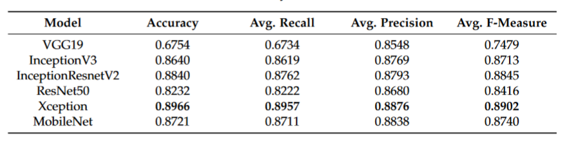
\includegraphics[width=1\textwidth]{2/figuras/Deep_Learning_Based_Transfer_Learning_imagen_01.png}
		\caption{Comparación de los resultados de los modelos utilizados. Fuente: \cite{jain2021deep}}
		\label{1:fig}
	\end{center}
\end{figure}






\subsection{Skin cancer classification via convolutional neural networks: systematic review of studies involving human experts \citep*{haggenmuller2021skin}}
\citeauthor{haggenmuller2021skin} realizaron un artículo de investigación el cual fue publicado en la revista «European Journal of Cancer» en el año 2021. Este fue titulado \citetitle{haggenmuller2021skin} la cual traducida al español significa «Clasificación del cáncer de piel mediante redes neuronales convolucionales: revisión sistemática de estudios en los que participan expertos humanos».

\subsubsection{Planteamiento del Problema y objetivo}
El estudio se enfoca en realizar un análisis de las investigaciones sobre estudios que involucran melanoma y evaluar su posible relevancia clínica mediante tres aspectos principales: características del conjunto de pruebas, prueba entorno y representatividad de los médicos participantes.

\subsubsection{Metodología empleada por los autores}
\newcommand{\TISCone}{Base de datos: Se examinaron los articulos publicados en las siguentes fuentes: PubMed, Medline y ScienceDirect en busca de estudios publicados entre 2017 y 2021.
	
}
\newcommand{\TISCtwo}{Requisitos para entrar a la investigación: Solo se incluían estudios se realizaba comparación directa de los resultados de la IA con médicos y que tenían como objetivo principal una clasificación diagnóstica.
}


\begin{itemize}
	\item \TISCone
	\item \TISCtwo
	%\item \TISCthree
	%\item \TISCfour
	
\end{itemize}

\subsubsection{Resultados obtenidos}
Solo un total de 19 estudios de lectores cumplieron los criterios de inclusión, de los cuales 11 enfoques basados en CNN abordaron la clasificación de imágenes dermatoscópicas, 6 se concentraron en la clasificación de imágenes clínicas, y 2 estudios dermatopatológicos utilizaron imágenes histopatológicas completas digitalizadas.



\begin{figure}[h]
	\begin{center}
		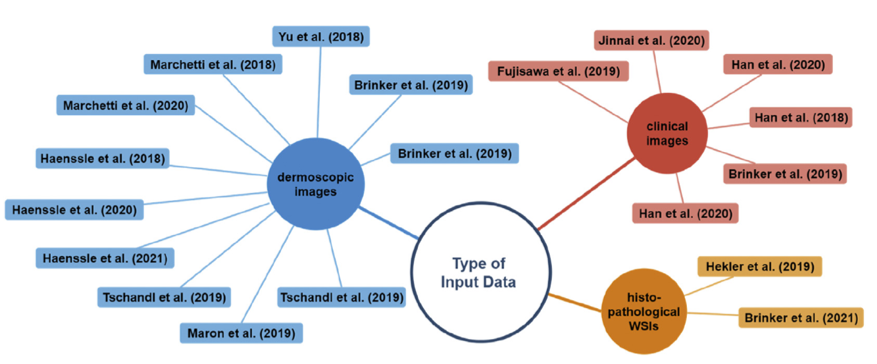
\includegraphics[width=1\textwidth]{2/figuras/Skin_cancer_classification _imagen_01.png}
		\caption{Represación de los 19 estudios. Fuente: \cite{haggenmuller2021skin}}
		\label{1:fig}
	\end{center}
\end{figure}





%% Problematica (2)


\subsection{An enhanced technique of skin cancer classification using deep convolutional neural network with transfer learning models \citep*{ali_2021enhanced}}
\citeauthor{ali_2021enhanced} realizaron un artículo de investigación el cual fue publicado en la revista «Machine Learning with Applications» en el año 2021 publicada por El servier. Este fue titulado \citetitle{ali_2021enhanced} la cual traducida al español significa «Una técnica mejorada de clasificación del cáncer de piel que utiliza una red neuronal convolucional profunda con modelos de aprendizaje por transferencia».

\subsubsection{Planteamiento del Problema y objetivo}
El cáncer de piel es uno de los tipos de cáncer de más rápido crecimiento y que puede causar la muerte, la realización de una detección temprana mejoraría significativamente las posibilidades de supervivencia del paciente. Por ello, el objetivo que se plantea es desarrollar un modelo de clasificación con la finalidad que distinguir las lesiones cutáneas benignas y malignas de forma precisa.


\begin{comment}
\subsubsection{Técnicas empleadas por los autores}
Los autores plantearon emplear diversas técnicas en las diferentes etapas de la metodología. En el caso del procesamiento, se centraron en la transformación de color para mejorar el contraste de la imagen y en un algoritmo de umbralización para detectar y clasificar artefactos de reflexión en las imágenes.

En la extracción de características, utilizaron ResNet50 para extraer características profundas para la clasificación de lesiones de piel.

En la implementación del modelo, emplearon una red neuronal convolucional profunda (DCNN) basada en aprendizaje profundo. Esta red neuronal es especialmente efectiva en tareas de procesamiento de imágenes, siendo capaz de aprender automáticamente características jerárquicas de las imágenes a través de capas convolucionales, lo que la hace ideal para problemas de clasificación de imágenes complejas como en este caso.
\end{comment}

\subsubsection{Metodología empleada por los autores}
\newcommand{\MEone}{ Adquisición de la data: Se uso una base de datos llamada HAM10000 compuesta por 10015 imágenes dermatoscópicas. Donde las imagenes fueron clasificados como malignas o benignas.
}
\newcommand{\MEtwo}{ Preprocesamiento: Se realizo diferentes tecnicas de pre-procesamiento como: reducción de datos, eliminación de burbujas de aire, ruido y artefactos, normalización de los datos y <<data augmentation>> . Esto con la finalidad de mejorar la tasa de clasificación del conjunto de datos en general. 
}

\newcommand{\MEthree}{ Extración de caracteristias: Se realizó una extracción de características para identificar y reconocer patrones en el conjunto de datos. 
}
\newcommand{\MEfour}{Implementación del modelo: Se entreno la red neuronal convolucional profunda (DCNN) y otro grupo de modelos para comprar AlexNet, ResNet, VGG-16, DenseNet, MobileNet.
Se hizo 3 diviciones del conjunto de datos: entrenamiento, validación y prueba de 2 formas distintas.

- 70\% entrenamiento, 20\% validación, 10\% prueba

- 80\% entrenamiento, 10\% validación, 10\% prueba
}


\begin{itemize}
	\item \MEone
	\item \MEtwo
	\item \MEthree
	\item \MEfour

\end{itemize}



\subsubsection{Resultados obtenidos}
Según el articulo el modelo propuesto DCNN fue el que obtuvo una precisión de clasificación del 93.16\% en el conjunto de entrenamiento y 91.93\% en el conjunto de prueba. A comparación del rendimiento que tuvieron los otros modelos de transfer learning como AlexNet, ResNet, VGG-16, DenseNet y MobileNet, los cuales fueron inferiores en términos de precisión, recall, puntaje F1 y tiempo de ejecución.

\begin{figure}[h]
	\begin{center}
		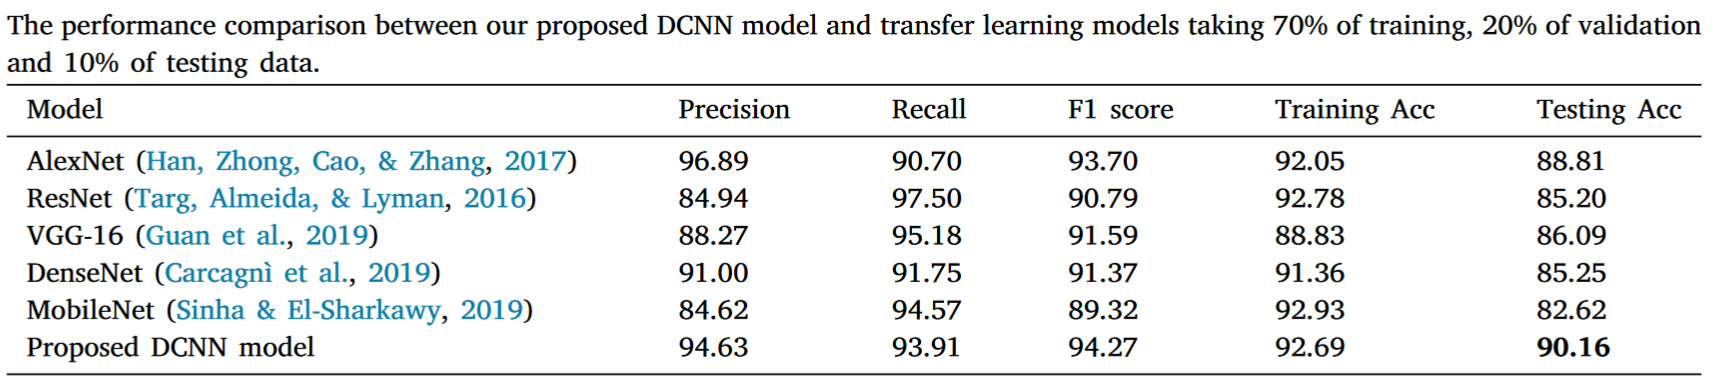
\includegraphics[width=1\textwidth]{2/figuras/Problematica_An_enhanced_tecniques_imagen_01.png}
		\caption{Resultados de modelo DCNN comparandolo con otros modelos Fuente: \cite{ali_2021enhanced}}
		\label{1:fig}
	\end{center}
\end{figure}




\subsection{Design of a tool for the classification of skin cancer imagesusing Deep Neural Networks (DNN) \citep*{vargas_2021diseno}}

\citeauthor{vargas_2021diseno} realizaron un artículo de investigación el cual fue publicado en la revista «Ciencia y Tecnología» en el año 2021 publicada por Universidad de Palermo (UP). Este fue titulado \citetitle{vargas_2021diseno}.


\subsubsection{Planteamiento del Problema y objetivo}
Los autores identifican que el cáncer de piel es una enfermedad común a nivel mundial que requiere un diagnóstico temprano para mejorar la calidad de vida de los pacientes. La clasificación automática de lesiones cutáneas presenta un reto debido a su amplia variedad y morfología. Por ende, el objetivo de la investigación es utilizar las ventajas del Deep Learning con la finalidad de desarrollar una red neuronal convolucional (CNN) entrenada para la clasificación de lesiones cutáneas benignas y malignas.


\begin{comment}
\subsubsection{Técnicas empleadas por los autores}
Los autores plantearon emplear diversas técnicas, entre ellas el uso de Data Augmentation para mejorar el tamaño y la calidad de los conjuntos de datos de entrenamiento, lo que ayudó a la construcción de modelos más efectivos.

Posteriormente, realizaron pruebas para ajustar la época, el tamaño del lote y la tasa de aprendizaje, con el fin de establecer valores óptimos y mejorar el rendimiento de los modelos durante el entrenamiento.

Finalmente, utilizaron K-fold Validation y F1 Score para evaluar el rendimiento de los modelos en la clasificación de lesiones benignas y malignas.
\end{comment}


\subsubsection{Metodología empleada por los autores}
\newcommand{\MEDone}{Recopilación de la data: Se uso dos bases de datos entre ellas HAM10000 compuesta por 10015 imágenes dermatoscópicas y ISIC (The International Skin Imaging Collaboration)la cual consta de 2357 imágenes de 226x226 píxeles de enfermedades oncológicas malignas y benignas.
}
\newcommand{\MEDtwo}{ Preprocesamiento:Se aplicó Transfer Learning para compartir características generales de bases de datos extensas, mejorando el rendimient. Haciendo uso de estrategias como Data Augmentation, ajuste de la tasa de aprendizaje y validación K-fold se implementaron para mejorar los modelos.
}

\newcommand{\MEDthree}{ Selección de arquitectura: Evaluaron diferentes arquitecturas como MobileNet V1, MobileNet V2, VGG19, VGG16, Inception V3, ResNet50. 
Al final se seleccionaron MobileNet V1 e Inception V3 como las arquitecturas más adecuadas
}

\newcommand{\MEDfour}{Implementación del modelo: Se implementaron diferentes versiones de modelos, desde el entrenamiento sin congelar capas hasta la adición de capas ocultas y estrategias de regularización. Para evaluar cual es el mejor modelo.
}


\begin{itemize}
	\item \MEDone
	\item \MEDtwo
	\item \MEDthree
	\item \MEDfour
\end{itemize}

\subsubsection{Resultados obtenidos}
El modelo MobileNet V1 alcanzó el mejor rendimiento a comparación de Inception V3. Este con un puntaje F1 del 91.06\%, una sensibilidad del 91.98\% y una tasa de falsos positivos del 9.65\%. 


\begin{figure}[h]
	\begin{center}
		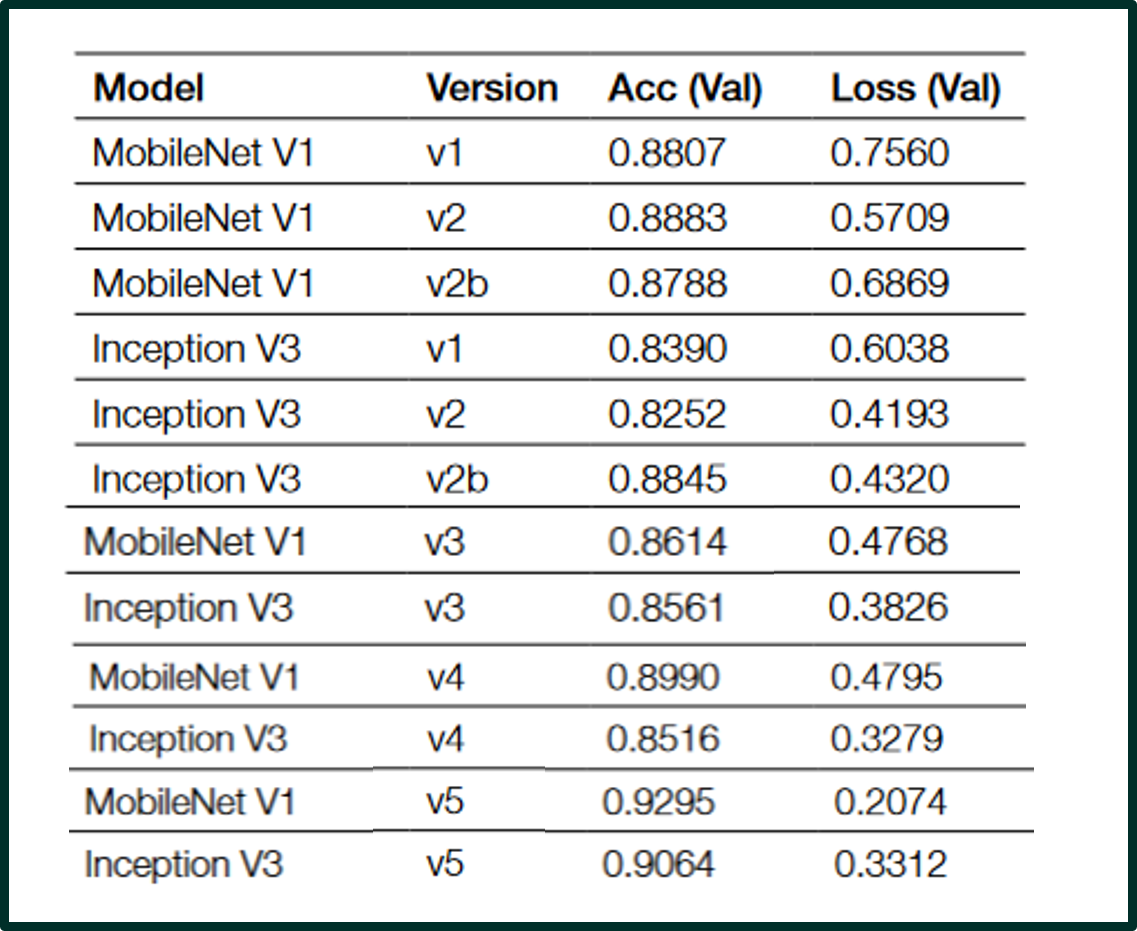
\includegraphics[width=0.6\textwidth]{2/figuras/Design_tool_the_classification_imagen_01.png}
		\caption{Comparacion de los resultados del modelo MobileNet V1 y Inception V3 con diferentes versiones. Fuente: \cite{vargas_2021diseno}}
		\label{1:fig}
	\end{center}
\end{figure}




%%% Tecnicas (6)

\subsection{Diagnosis of skin cancer using machine learning techniques \citep*{murugan_2021diagnosis}}

\citeauthor{murugan_2021diagnosis} realizaron un artículo de investigación el cual fue publicado en la revista «Microprocessors and Microsystems» en el año 2021. Este fue titulado \citetitle{murugan_2021diagnosis} la cual traducida al español significa «Diagnóstico del cáncer de piel mediante técnicas de aprendizaje automático».



\subsubsection{Planteamiento del Problema y objetivo}
 El artículo destaca el problema de la detección temprana del cáncer de piel, ya que la piel desempeña un papel vital en el cuerpo humano y cualquier cambio en su funcionamiento puede afectar significativamente la salud general.

Enfocandose que las lesiones cutáneas que son signos clínicos importantes de enfermedades de la piel, como el melanoma y el carcinoma de células basales. Estos son una forma peligrosa de cáncer que puede propagarse rápidamente si no se detecta a tiempo

Por ende, el objetivo principal del estudio es desarrollar un sistema de identificación de enfermedades de la piel basado en imágenes de la piel. Empleando técnicas de aprendizaje automático como SVM, PNN y Random Forest

\begin{comment}
\subsubsection{Técnicas empleadas por los autores}
Según el articulo se realizan comparaciones entre diversas tecnicas para confirmar cual es la mejor.

En el caso la extraccion de caracteristicas: se usaron GLCM, Moment Invariants and GLRLM.

Aquí se presentan algunas de sus ecuaciones:
%%%Ecuacion
\begin{equation}  
	\label{eq:GLCM}
	GLCM = \sum_{x} \sum_{y} (x + a)^p \cdot (y + b)^q \, f(x, y)
\end{equation}


\begin{equation}
		\label{eq:Moment Invariants}
Moment Invariants = \sum_{x=0}^{M-1} \sum_{y=0}^{M-1} x^p \cdot y^q \, f(x, y) \quad \text{para} \quad p, q = 0, 1, 2, 3
\end{equation}


Para comprobar cual modelo obtiene mejores descriptores de las imágenes de lesiones cutáneas. 

Luego, emplearon varios clasificadores de aprendizaje automático: PNN, SVM, Random Forest y SVM + RF (Máquinas de Vectores de Soporte (SVM), Redes Neuronales Probabilísticas (PNN), Bosques Aleatorios (RF) y una combinación de SVM y RF). Para identificar y clasificar diferentes tipos de lesiones de piel.
\end{comment}


\subsubsection{Metodología empleada por los autores}
\newcommand{\MEDSone}{ Recopilación de la data: En este caso no se especifica el tamaño o la fuente exacta del conjunto de datos. Sin embargo, menciona que se empleó un conjunto de datos de imágenes dermoscópicas para identificar y clasificar diferentes tipos de lesiones de piel, como lentigo simple, melanoma, carcinoma basocelular, entre otros.
	
}
\newcommand{\MEDStwo}{ Preprocesamiento: Se dividio en dos etapas: 

- Primera etapa: Removieron el ruido de las imágenes para eliminar pelos y burbujas que pueden afectar la extracción de características,  utilizando un filtro de mediana.

- Segunda etapa: Uso del algoritmo de segmentación Mean Shift para separar la región de interés (ROI) que contiene la lesión del fondo de la imagen.
	
}

\newcommand{\MEDSthree}{ Extracción de características: Uso de tres técnicas para la extracción de características de las imágenes: 
	
- Gray Level Co-Occurrence Matrix (GLCM)

- Moment Invariants(MI)

- Gray Level Run Length Matrix (GLRLM)

}
\newcommand{\MEDSfour}{Implementación del modelo: 
	Se aplican técnicas de clasificación como Máquinas de Vectores de Soporte (SVM), Redes Neuronales Probabilísticas y Bosques Aleatorios, así como la combinación de SVM y Random Forest, con las distintas técnicas para las características extraídas.
}


\begin{itemize}
	\item \MEDSone
	\item \MEDStwo
	\item \MEDSthree
	\item \MEDSfour
\end{itemize}


\subsubsection{Resultados obtenidos}
El rendimiento de los modelos que se emplearon se evaluó en términos de métricas como precisión, sensibilidad y especificidad
Dado como resultado que el mejor clasificador fue la combinación de SVM y Random Forest (SVM+RF) usando un extractor de características GLCM dando un accuracy de 89.31\% 
\begin{figure}[h]
	\begin{center}
		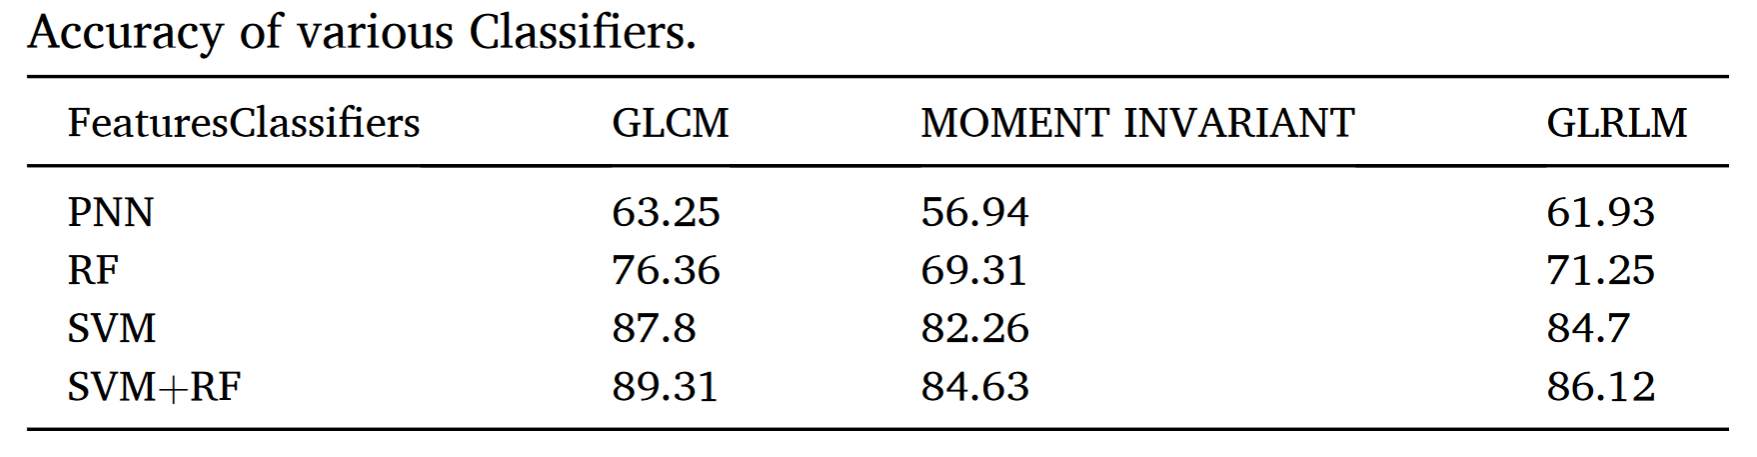
\includegraphics[width=0.6\textwidth]{2/figuras/Tecnica_Diagnosis_skin_cancer_imagen_01.png}
		\caption{Comparación de los modelo empleados con las  tres técnicas para la extracción de características. Fuente: \cite{murugan_2021diagnosis}}
		\label{1:fig}
	\end{center}
\end{figure}






\subsection{Multiclass skin cancer classification using EfficientNets – a first step towards preventing skin cancer \citep*{ali_2022multiclass}}
\citeauthor{ali_2022multiclass} realizaron un artículo de investigación el cual fue publicado en la revista «Neuroscience Informatics» en el año 2022. Este fue titulado \citetitle{ali_2022multiclass} la cual traducida al español significa «Clasificación de cáncer de piel multiclase utilizando redes eficientes: un primer paso para prevenir el cáncer de piel».




\subsubsection{Planteamiento del Problema y objetivo}

La clasificación del cáncer de piel presenta una alta dificultad debido a la variabilidad en la apariencia de sus diversas categorías diagnósticas. Aunque los dermatólogos suelen diagnosticar esta enfermedad visualmente, estudios recientes han demostrado que el uso de la  tecnologia pueden superar ayudar a los dermatólogos.

El objetivo principal es desarrollar un sistema de clasificación de cáncer de piel utilizando la técnica de transfer learning en redes neuronales convolucionales pre-entrenadas.

\begin{comment}
\subsubsection{Técnicas empleadas por los autores}
Redes EfficientNets: Se utilizaron los modelos EfficientNets B0-B7 preentrenados con pesos de ImageNet. Estos modelos se ajustaron finamente (fine-tuning) con el conjunto de datos.

Detección de características: Se extrajeron características utilizando redes neuronales convolucionales (CNN) preentrenadas.

Transfer learning: Se aplicó transfer learning para entrenar el conjunto de datos en los pesos preentrenados de ImageNet y ajustar finamente las CNN.

Optimización de hiperparámetros: Se ajustaron hiperparámetros como las tasas de aprendizaje cíclico para entrenar las redes neuronales.

Métricas de evaluación: Se utilizaron métricas como precisión, recall, exactitud y puntaje F1 para evaluar el rendimiento de los modelos. También se emplearon matrices de confusión.
\end{comment}


\subsubsection{Metodología empleada por los autores}

\newcommand{\MEDMone}{Adquisición de la data: Se uso una base de datos llamada HAM10000 compuesta por 10015 imágenes dermatoscópicas. De donde se dibirieron las imagenes en siete difetentes tipos de cancer de piel}

\newcommand{\MEDMtwo}{ Preprocesamiento: Primero se elimino la precencia de elemenotos no relevantes, en este caso los pelos que aparecia en la mayoria de las imagenes. Continuando con la redimencioón de las imagenes de acuerdo con los requerimientos de cada variante de  EfficientNet (B0-B7). Finalizando con el aumento de datos para tener la misma cantidad en cada partición.}

\newcommand{\MEDMthree}{Entrenamiento y validación:
 Los modelos se entrenaron y validaron utilizando técnicas como k-Fold Cross-Validation y se evaluaron con métricas como precisión, recall, exactitud y puntaje F1.}



\begin{itemize}
	\item \MEDMone
	\item \MEDMtwo
	\item \MEDMthree
	
\end{itemize}

\subsubsection{Resultados obtenidos}

Según la tabla de resultados se concluyó que  el modelo EfficientNet B4 logró los mejores resultados con un puntaje F1 del 87\% y una exactitud de clasificación Top-1 del 87.91\%, destacando su eficacia en la clasificación multiclase del cáncer de piel en el conjunto de datos HAM10000.

\begin{figure}[h]
	\begin{center}
		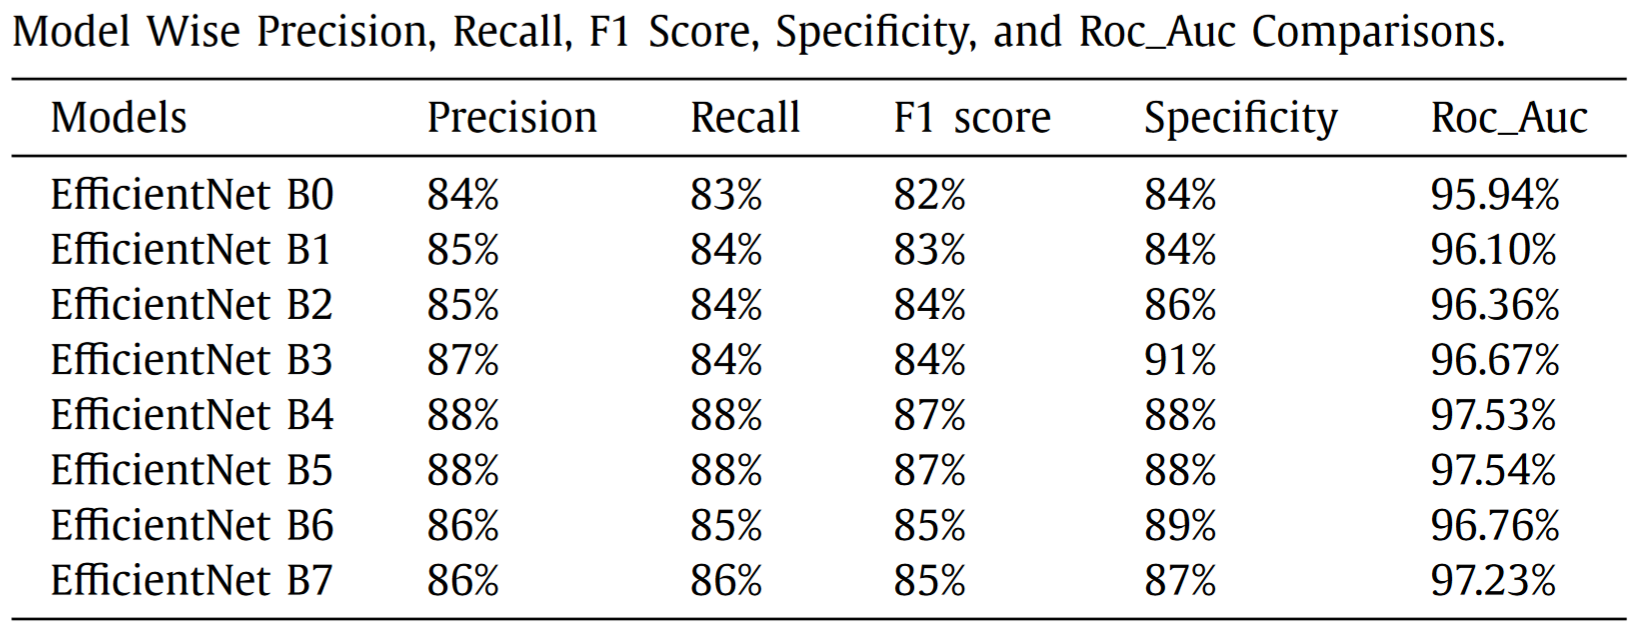
\includegraphics[width=0.7\textwidth]{2/figuras/Multiclass_skin_cancer_imagen_01.png}
		\caption{Comparación de los modelo empleados con las  tres técnicas para la extracción de características. Fuente: \cite{ali_2022multiclass}}
		\label{1:fig}
	\end{center}
\end{figure}

\subsection{Skin cancer classification using explainable artificial intelligence on pre-extracted image features \citep*{khater2023skin}}
\citeauthor{khater2023skin} realizaron un artículo de investigación el cual fue publicado en la revista «Intelligent Systems with Applications» en el año 2023. Este fue titulado \citetitle{khater2023skin} la cual traducida al español significa «Clasificación del cáncer de piel utilizando inteligencia artificial explicable en características de imágenes previamente extraídas».

\subsubsection{Planteamiento del Problema y objetivo}
Los autores plantearon la necesidad de desarrollar un modelo de clasificación de cáncer de piel que no solo sea preciso sino también explicativo. Esto usando inteligencia artificial explicativa (XAI) para clasificar lesiones de piel en tres clases: nevus típico, nevus atípico y melanoma


\begin{comment}
\subsubsection{Técnicas empleadas por los autores}
Se emplearon varias técnicas de aprendizaje automático (ML) y de inteligencia artificial explicable (XAI) para clasificar el cáncer de piel, las cuales fueron.

Técnicas de aprendizaje automático (ML): XGBoost, árboles de decisión, random forest y KNN(K-Nearest Neighbors),

Inteligencia artificial explicable (XAI): SHAP (Shapley Additive Explanations), Permutation importance, Partial dependence plot y Local Interpretable Model-agnostic methods(LIME)

\end{comment}

\subsubsection{Metodología empleada por los autores}

\newcommand{\TPSCone}{Recopilación de la data: Se uso un conjunto de datos PH2(recopilación de datos en el departamento de dermatología del Hospital Pedro Hispano)
Este conjunto de datos contiene imágenes dermatoscopia con siete características de entrada y una característica de salida.

}

\newcommand{\TPSCtwo}{ Preprocesamiento: El conjunto de datos se sometio a un proceso de preprocesamiento para mejorar su calidad y preparación para el análisis.}

\newcommand{\TPSCthree}{Extracción de características: Se extrajeron características clave de las imágenes
% Estas características incluyen asimetría, pigment network, dots/globules, streaks, regression areas, blue-white veil regions, y el número de colores presentes en el cáncer de piel.
y usando el método chi-cuadrado se estimo la importancia de cada una de las características y se selecciono las más significativas.
}


\newcommand{\TPSCfour}{ Entrenamiento de modelos de ML: Se entrenaron varios algoritmos de aprendizaje automático (ML) utilizando las características pre-extraídas. Los algoritmos incluyen KNN, XG-boost, árboles de decisión, y bosques aleatorios.
}

\begin{itemize}
	\item \TPSCone
	\item \TPSCtwo
	\item \TPSCthree
	\item \TPSCfour
	
\end{itemize}



\subsubsection{Resultados obtenidos}
El modelo XG-boost como para el Random Forest alcanzó una precisión del min de 94\%. 


\begin{figure}[h]
	\begin{center}
		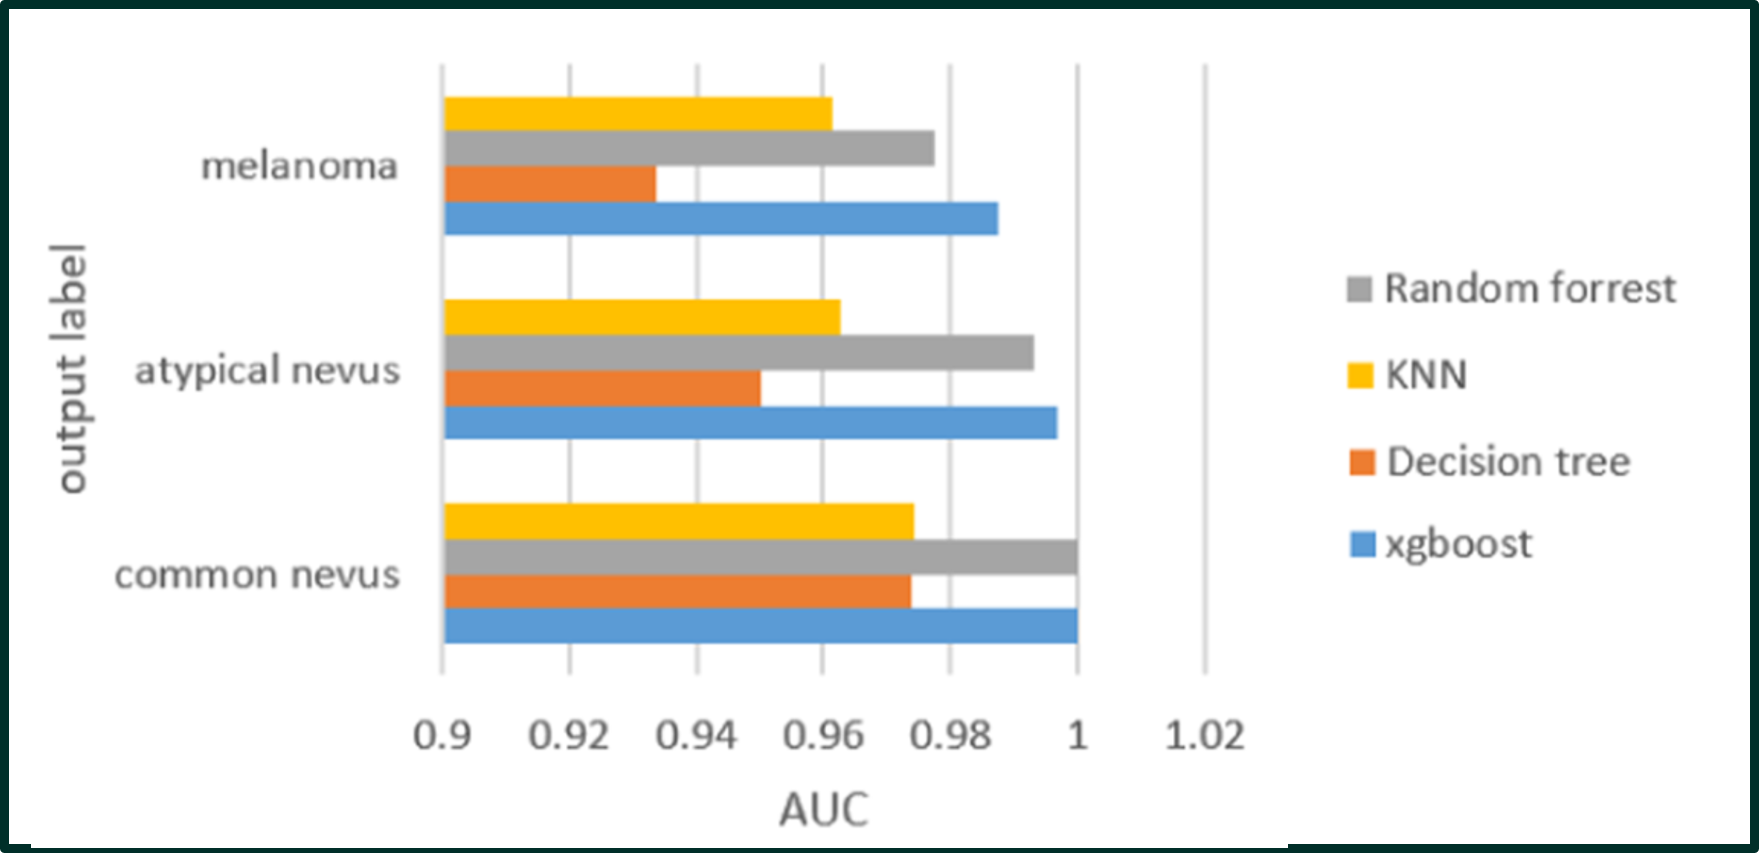
\includegraphics[width=0.5\textwidth]{2/figuras/Skin_cancer_classification_imagen_01.png}
		\caption{Comparación de los modelo empleados con las  tres técnicas para la extracción de características. Fuente: \cite{ali_2022multiclass}}
		\label{1:fig}
	\end{center}
\end{figure}





\subsection{An improved transformer network for skin cancer classification \citep*{xin2022improved}}
\citeauthor{xin2022improved} realizaron un artículo de investigación el cual fue publicado en la revista «Computers in Biology and Medicine» en el año 2022. Este fue titulado \citetitle{xin2022improved} la cual traducida al español significa «Una red de transformadores mejorada para la clasificación del cáncer de piel».


\subsubsection{Planteamiento del Problema y objetivo}

El artículo se centra en la necesidad de mejorar la clasificación de imágenes de cáncer de piel para su diagnóstico temprano. Debido al aumento de su incidencia en todo el mundo, lo que representa una gran amenaza para la salud humana. 
En el documento se propone desarrollar un modelo de red transformadora mejorada que pueda lograr una mayor precisión en la clasificación de diferentes tipos de cáncer de piel, mediante el uso de una red neuronal transformadora de visión (VIT).





\subsubsection{Metodología empleada por los autores}
\newcommand{\TPACone}{Recopilación de la data: Se uso un conjunto de datos HAM10000 del archivo ISIC, que incluye siete clases exclusivas de cáncer de piel y recolección de imágenes de cáncer de piel de pacientes hospitalarios mediante dermatoscopia, incluyendo tres tipos de cáncer de piel típicos.	
}

\newcommand{\TPACtwo}{Preprocesamiento: Se llevaron a cabo tres trabajos con la base de datos. Primero, la normalización, para limitar los datos preprocesados a un rango específico y eliminar singularidades y efectos adversos causados por los datos de muestra. Segundo, el aumento de datos, que incluyó técnicas como volteo horizontal y vertical, recorte aleatorio, rotación aleatoria y ajuste de color para mejorar la diversidad de los datos. Por ultimo, el muestreo equilibrado, para garantizar una distribución equitativa de las clases en el conjunto de datos. }

\newcommand{\TPACthree}{Extracción de características: Uso de un transformador de visión multi-escala para dividir una imagen en diferentes tipos de parches. Permitiendo capturar características a múltiples escalas preservando la estructura de los bloques de imagen adyacentes.
}


\newcommand{\TPACfour}{ Entrenamiento de modelos: Se evaluó el modelo propuesto Modelo VIT (Vision Transformer) utilizando métricas como precisión, recuperación, puntaje F1 y AUC en los conjuntos de datos HAM10000 y el conjunto de datos clínico recopilado.
Despues se comparó el rendimiento del modelo propuesto con otros modelos existentes los cuales fueron oft attention network, Ensembles of multi-resolution (EfficientNets), Single model deep learning, Data augmentation for skin classification, Two path CNN model, Deep CNN (Baseline), MobileNetV2, ResNet50, InceptionV2. Con la finalidad de demostrar su eficacia y generalización.	
}

\begin{itemize}
	\item \TPACone
	\item \TPACtwo
	\item \TPACthree
	\item \TPACfour
	
\end{itemize}


\subsubsection{Resultados obtenidos}
El modelo VIT logró un AUC de 0.987, una precisión de 0.941 en el conjunto de datos clínicos recopilados y una precisión de 0.943 en el conjunto de datos HAM10000, superando en 0.3\%, 4.6\%, 1.3\%, 1.2\% y 0.8\% respectivamente a otros modelos.

\begin{figure}[h]
	\begin{center}
		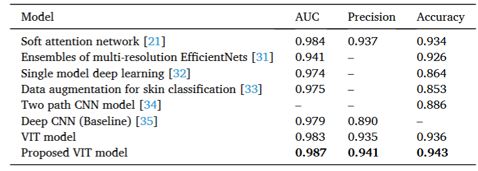
\includegraphics[width=0.5\textwidth]{2/figuras/An_improved_transformer_network _imagen_01.png}
		\caption{Resultados de los Modelo empleados. Fuente: \cite{xin2022improved}}
		\label{1:fig}
	\end{center}
\end{figure}




\subsection{Uncertainty quantification in skin cancer classification using three-way decision-based Bayesian deep learning \citep*{abdar2021uncertainty}}
\citeauthor{abdar2021uncertainty} realizaron un artículo de investigación el cual fue publicado en la revista «Computers in Biology and Medicine» en el año 2022. Este fue titulado \citetitle{abdar2021uncertainty} la cual traducida al español significa «Cuantificación de la incertidumbre en la clasificación del cáncer de piel mediante aprendizaje profundo bayesiano de tres vías basado en decisiones».
\subsubsection{Planteamiento del Problema y objetivo}
Los autores se enfocan en la necesidad de cuantificar la incertidumbre en la clasificación de imágenes de cáncer de piel utilizando deep learning, enfocado en la toma de decisiones médicas. Por ello, su objetivo principal es diseñar y validar un nuevo modelo de cuantificación de incertidumbre basado en la teoría de la decisión trinaria y deep learning  para mejorar la confiabilidad y la conciencia de la incertidumbre en la clasificación de imágenes médicas.

\subsubsection{Metodología empleada por los autores}
\newcommand{\TUQSone}{Recopilación de Datos: Los autores recopilaron dos conjuntos de datos de 2 partes: uno de Kaggle y otro del ISIC 2019. Los cuales se realizo un preprocesamiento para preparar las imágenes para su análisis.
}

\newcommand{\TUQStwo}{ Selección de Arquitecturas de Deep Learning: Se seleccionaron cuatro arquitecturas de deep learning conocidas (ResNet152V2, MobileNetV2, DenseNet201 e InceptionResNetV2) como modelos preentrenados en ImageNet. Donde se uso la Optimización Bayesiana (BO) para determinar los mejores valores de hiperparámetros para cada arquitectura y conjunto de datos.
 }

\newcommand{\TUQSthree}{Modelo de tres fases: Se implementó un modelo de tres fases que incluye la detección de muestras inciertas, la clasificación inicial y la clasificación final. Se utilizó un modelo de decisión basado en tres vías (TWDBDL) que combina métodos de incertidumbre con redes neuronales profundas para mejorar la clasificación de cáncer de piel. En la segunda fase, se empleó un modelo de conjunto (EMC) con diferentes arquitecturas de redes neuronales para procesar los datasets
La TWD se utilizó para mejorar la precisión y confiabilidad de las predicciones del modelo al integrarla con las técnicas de cuantificación de incertidumbre en el modelo de aprendizaje profundo.
}

\begin{itemize}
	\item \TUQSone
	\item \TUQStwo
	\item \TUQSthree

\end{itemize}



\subsubsection{Resultados obtenidos}
Para el primer dataset:En la primera fase, el método DE (Deep Ensemble) aplicado a modelos como ResNet152V2, DenseNet201, InceptionResNetV2 y MobileNetV2 logró una precisión del 87.55\%. En la segunda fase, el método EMC (Ensemble Monte Carlo Dropout) obtuvo la mejor AUC, mientras que la precisión de la clase 1 (casos malignos) fue meno

Para el segundo dataset: En la primera fase, el método EMC aplicado a modelos como ResNet152V2, DenseNet201 y DenseNet201 obtuvo una precisión del 89.39\% y un F1-score del 92\%. En la segunda fase, también se utilizó EMC. En la fase final, la precisión de la clase 0 (casos de melanoma) se mantuvo estable, mientras que la precisión de la clase 1 (casos no melanoma) aumentó.

En resumen el modelo TWDBDL propuesto logró buenos resultados de precisión, F1-score y AUC en la clasificación de cáncer de piel, especialmente al detectar y manejar adecuadamente las muestras inciertas.

\begin{figure}[h]
	\begin{center}
		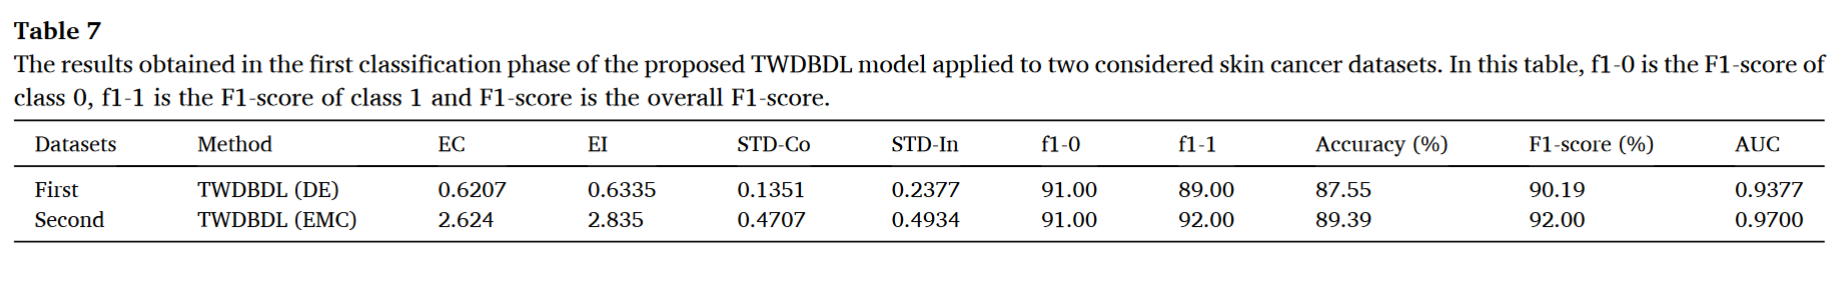
\includegraphics[width=0.8\textwidth]{2/figuras/Uncertainty_quantification_skin _imagen_01.png}
		\caption{Resultados de los Modelo empleados. Fuente: \cite{abdar2021uncertainty}}
		\label{1:fig}
	\end{center}
\end{figure}


\subsection{A multi-class skin Cancer classification using deep convolutional neural networks \citep*{chaturvedi2020multi}}
\citeauthor{chaturvedi2020multi} realizaron un artículo de investigación el cual fue publicado en «Springer Science+Business Media, LLC, part of Springer Nature 2020» en el año 2020. Este fue titulado \citetitle{chaturvedi2020multi} la cual traducida al español significa «Una clasificación de cáncer de piel de múltiples clases utilizando redes neuronales convolucionales profundasl».

\subsubsection{Planteamiento del Problema y objetivo}


\subsubsection{Metodología empleada por los autores}
\newcommand{\TUAMCone}{Recopilación de la data: Se uso los siguetes conjustos de datos: ISIC2017, ISIC2018, y HAM10000. Donde se realizó ajustes para asegurar que los datos estén en un formato adecuado para el entrenamiento de los modelos.
}

\newcommand{\TUAMCtwo}{Implementación de Modelos: Se utilizan diferentes arquitecturas de redes neuronales convolucionales profundas como Xception, InceptionV3, ResNetXt101, InceptionResNetV2 y NASNetLarge para la clasificación de siete tipos de cáncer de piel. }

\newcommand{\TUAMCthree}{Optimización de Modelos(hiperparametos): Se emplean optimizadores como stochastic gradient descent with momentum (SGDM) y adaptive moment estimation (Adam) para ajustar los modelos y minimizar la función de pérdida.
}


\newcommand{\TUAMCfour}{Evaluación de Desempeño: Se evalúa el desempeño de los modelos en un conjunto de validación de 1103 imágenes, calculando métricas como recall, precision, exactitud (accuracy) y F1-score para cada modelo y para las combinaciones de modelos de ensemble.
	
}

\begin{itemize}
	\item \TUAMCone
	\item \TUAMCtwo
	\item \TUAMCthree
	\item \TUAMCfour
\end{itemize}

\subsubsection{Resultados obtenidos}

El accuracy más alto se logró con el modelo ResNeXt101 y InceptionResNetV2, en ambos casos con un 93.20%.
No obstante ResNeXt101 consiguio una mejor precisión que InceptionResNetV2 por una diferencia de 1\%.

\begin{figure}[h]
	\begin{center}
		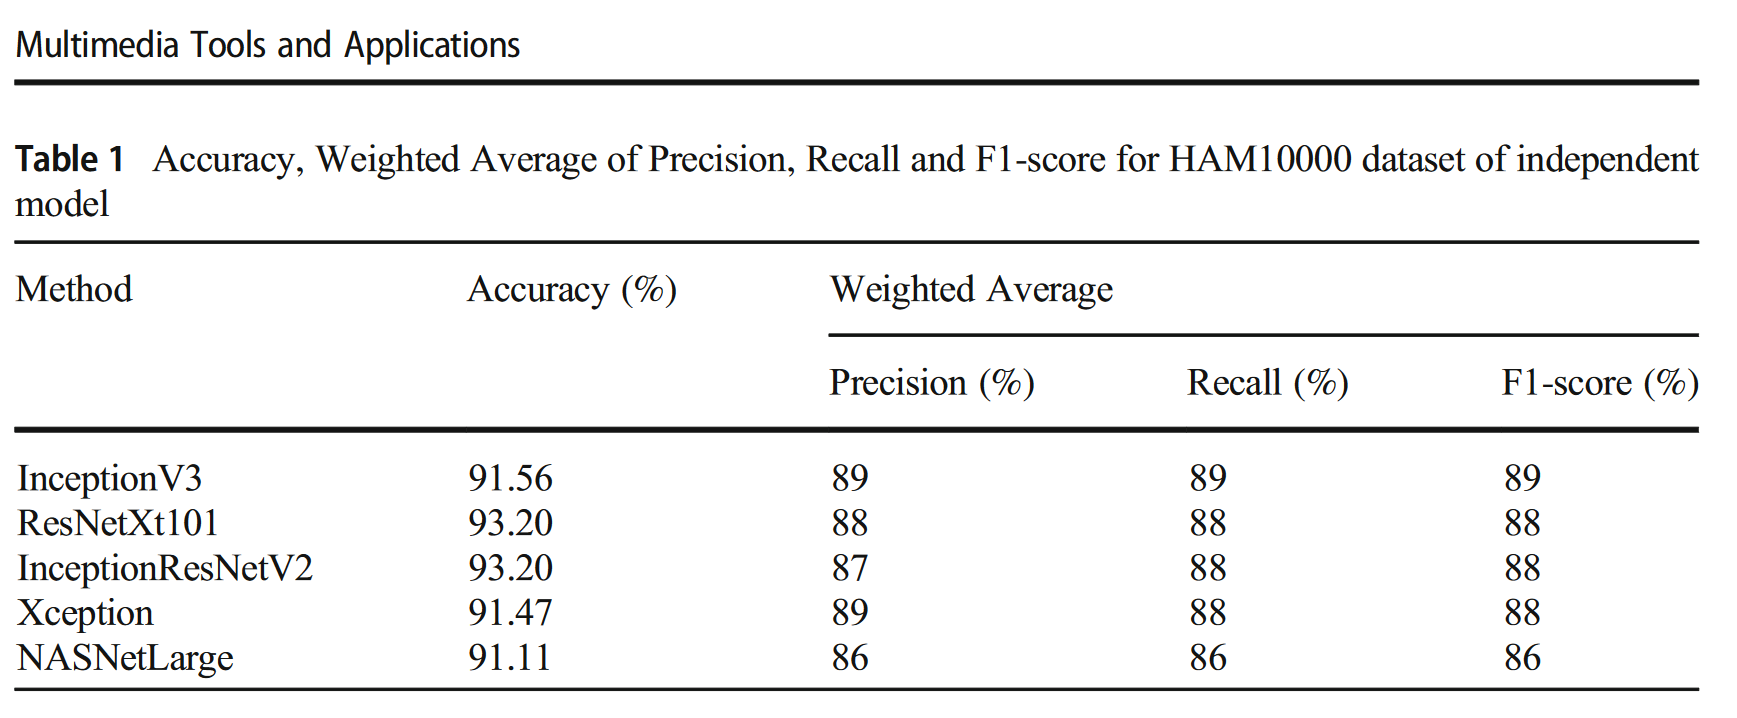
\includegraphics[width=0.8\textwidth]{2/figuras/An_improved_network_skin_cancer_classification_imagen_01.png}
		\caption{Resultados de los Modelo empleados. Fuente: \cite{chaturvedi2020multi}}
		\label{1:fig}
	\end{center}
\end{figure}





